\chapter{Module \& Detector Development}
\label{ch:development}

This chapter provides a few brief recipes for developing new simulation modules and detector models for the \apsq framework.
Before starting the development, the \file{CONTRIBUTING.md} file in the repository should be consulted for further information on the development process, code contributions and the preferred coding style for \apsq.

\section{General Rules}

The following general rules, also know as \textswab{Koen's: Coding Commandments:} should be followed when working on the code of the \apsq framework.

\begin{figure}[H]
  \centering
  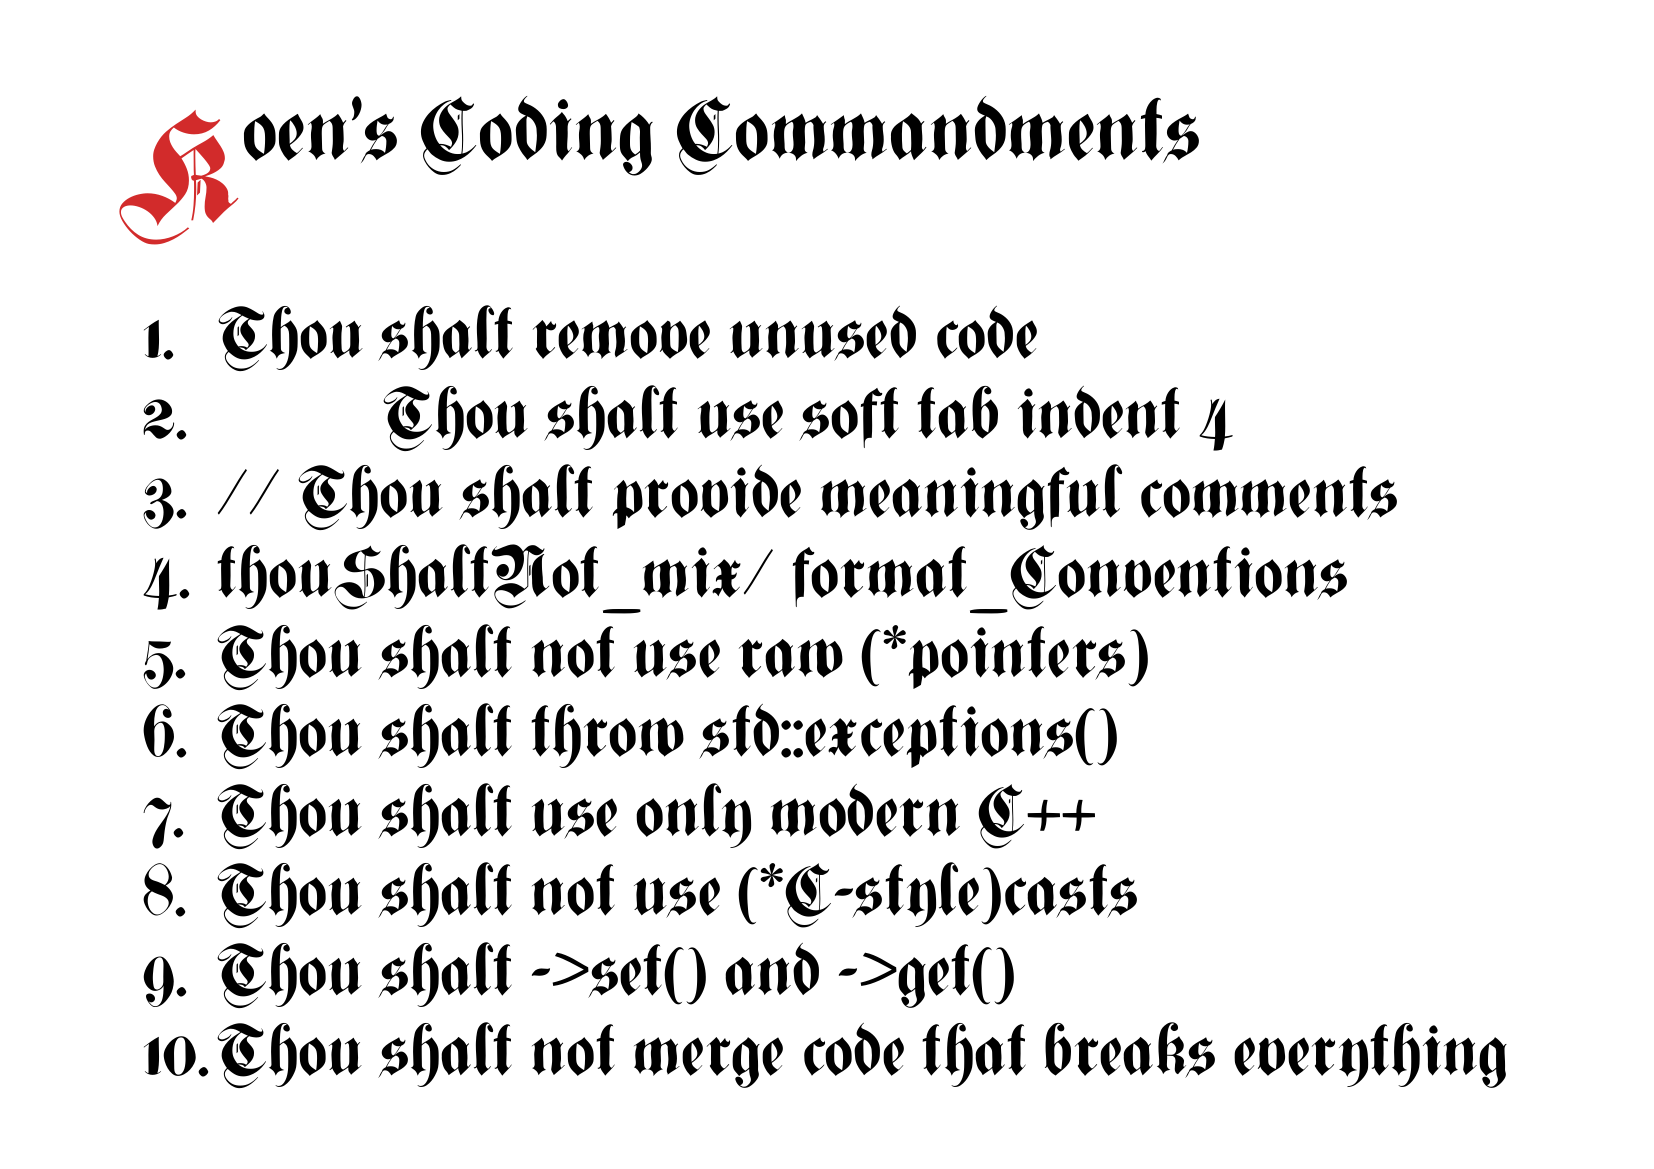
\includegraphics[width=\textwidth]{coding_commandments.png}
\end{figure}

\section{Coding and Naming Conventions}

The code base of the \apsq is well-documented and follows concise rules on naming schemes and coding conventions.
This enables maintaining a high quality of code and ensures maintainability over a longer period of time.
In the following, some of the most important conventions are described.
In case of doubt, existing code should be used to infer the coding style from.

\subsection{Naming Schemes}

The following coding and naming conventions should be adhered to when writing code which eventually should be merged into the main repository.

\begin{description}
    \item[Namespace] The \parameter{allpix} namespace is to be used for all classes which are part of the framework, nested namespaces may be defined. It is encouraged to make use of \command{using namespace allpix;} in implementation files only for this namespace. Especially the namespace \parameter{std} should always be referred to directly at the function to be called, e.g.\ \command{std::string test}. In a few other cases, such as \parameter{ROOT::Math}, the \command{using} directive may be used to improve readability of the code.

    \item[Class names] Class names are typeset in CamelCase, starting with a capital letter, e.g.\ \command{class ModuleManager{}}. Every class should provide sensible Doxygen documentation for the class itself as well as for all member functions.

    \item[Member functions] Naming conventions are different for public and private class members. Public member function names are typeset as camelCase names without underscores, e.g.\ \command{getElectricFieldType()}. Private member functions use lower-case names, separating individual words by an underscore, e.g.\ \command{create_detector_modules(...)}. This allows to visually distinguish between public and restricted access when reading code.

    In general, public member function names should follow the \command{get}/\command{set} convention, i.e.\ functions which retrieve information and alter the state of an object should be marked accordingly. Getter functions should be made \parameter{const} where possible to allow usage of constant objects of the respective class.

    \item[Member variables] Member variables of classes should always be private and accessed only via respective public member functions. This allows to change the class implementation and its internal members without requiring to rewrite code which accesses them. Member names should be typeset in lower-case letters, a trailing underscore is used to mark them as member variables, e.g.\ \parameter{bool terminate_}. This immediately sets them apart from local variables declared within a function.
\end{description}

\subsection{Formatting}

A set of formatting rules is applied to the code base in order to avoid unnecessary changes from different editors and to maintain readable code.
The formatting rules are defined in the \file{.clang-format} file in the repository in machine-readable form (for \command{clang-format}, that is) but can be summarized as follows:

\begin{itemize}
  \item The column width should be 125 characters, with a line break afterwards.
  \item New scopes are indented by four whitespaces, no tab characters are to be used.
  \item Namespaces are indented just as other code is.
  \item No spaces should be introduced before parentheses ().
  \item Included header files should be sorted alphabetically.
  \item The pointer asterisk should be left-aligned, i.e. \command{int* foo} instead of \command{int *foo}.
\end{itemize}
The continuous integration automatically checks if the code adheres to the defined format as described in Section~\ref{sec:ci}.

\section{Implementing a New Module}
\label{sec:building_new_module}

Owing to its modular structure, the functionality of the \apsq can easily be extended by adding additional modules which can be placed in the simulation chain.
Since the framework serves a wide

Before starting the development of a new module, it is essential to carefully read the documentation of the framework module manager which can be found in Section~\ref{sec:module_manager}.

, the information about the directory structure in Section~\ref{sec:module_files} and the details of the module structure in Section~\ref{sec:module_structure} before creating a new module.
Thereafter, the steps below should provide enough details for starting a new module, hereafter called \parameter{ModuleName}:
\begin{enumerate}
    \item Run the module initialization script at \file{etc/scripts/make_module.sh} in the repository.
    The script will ask for the name of the model and the type (unique or detector-specific).
    It creates the directory with a minimal example to get started together with the rough outline of its documentation in \textit{README.md}.
    \item Before starting to implement the actual module, it is recommended to update the introductory documentation in \textit{README.md}.
    No additional documentation in LaTeX has to be provided, as this Markdown-formatted file~\cite{markdown} is automatically converted and included in the user manual.
    Formulae can be included by enclosure in Dollar-backtick markers, i.e. `$` E(z) = 0`$`.
    The Doxygen documentation in \textit{\texttt{ModuleName}.hpp} should also be extended to provide a basic description of the module.
    \item Finally, the constructor and \command{init}, \command{run} and/or \command{finalize} methods can be written, depending on the requirements of the new module.
\end{enumerate}

After this, it is up to the developer to implement all required functionality.

It should be kept in mind that writing more generic modules, which are not tied to a specific detector type or simulation, will allow other users to benefit from the development.
Furthermore, it may be beneficial to split up modules to support the modular design of \apsq.
Additional sources of documentation which may be useful during the development of a module include:
\begin{itemize}
\item The framework documentation in Chapter~\ref{ch:framework} for an introduction to the different parts of the framework.
\item The module documentation in Chapter~\ref{ch:modules} for a description of the functionality of other modules already implemented, and to look for similar modules which can help during development.
\item The Doxygen (core) reference documentation included in the framework~\cite{ap2-doxygen}.
\item The latest version of the source code of all modules and the \apsq core itself.
\end{itemize}

Any module potentially useful for other users should be contributed back to the main repository after is has been validated.
It is strongly encouraged to send a merge-request through the mechanism provided by the software repository~\cite{ap2-repo}.

\subsection{Files of a Module}
\label{sec:module_files}
Every module directory should at minimum contain the following documents (with \texttt{ModuleName} replaced by the name of the module):
\begin{itemize}
\item \textbf{CMakeLists.txt}: The build script to load the dependencies and define the source files of the library.
\item \textbf{README.md}: Full documentation of the module.
\item \textbf{\textit{ModuleName}Module.hpp}: The header file of the module.
\item \textbf{\textit{ModuleName}Module.cpp}: The implementation file of the module.
\end{itemize}
These files are discussed in more detail below.
By default, all modules added to the \textit{src/modules/} directory will be built automatically by CMake.
If a module depends on additional packages which not every user may have installed, one can consider adding the following line to the top of the module's \textit{CMakeLists.txt}:
\begin{minted}[frame=single,framesep=3pt,breaklines=true,tabsize=2,linenos]{cmake}
ALLPIX_ENABLE_DEFAULT(OFF)
\end{minted}

General guidelines and instructions for implementing new modules are provided in Section~\ref{sec:building_new_module}.

\paragraph{CMakeLists.txt}
Contains the build description of the module with the following components:
\begin{enumerate}
\item On the first line either \parameter{ALLPIX_DETECTOR_MODULE(MODULE_NAME)} or \parameter{ALLPIX_UNIQUE_MODULE(MODULE_NAME)} depending on the type of module defined.
The internal name of the module is automatically saved in the variable \parameter{${MODULE_NAME}} which should be used as an argument to other functions.
Another name can be used by overwriting the variable content, but in the examples below, \parameter{${MODULE_NAME}} is used exclusively and is the preferred method of implementation.
\item The following lines should contain the logic to load possible dependencies of the module (below is an example to load Geant4).
Only ROOT is automatically included and linked to the module.
\item A line with \texttt{\textbf{ALLPIX\_MODULE\_SOURCES(\$\{MODULE\_NAME\} \textit{sources})}} defines the module source files. Here, \texttt{sources} should be replaced by a list of all source files relevant to this module.
\item Possible lines to include additional directories and to link libraries for dependencies loaded earlier.
\item A line containing \parameter{ALLPIX_MODULE_INSTALL(${MODULE_NAME})} to set up the required target for the module to be installed to.
\end{enumerate}

A simple CMakeLists.txt for a module named \parameter{Test} which requires Geant4 is provided below as an example.
\vspace{5pt}

\begin{minted}[frame=single,framesep=3pt,breaklines=true,tabsize=2,linenos]{cmake}
# Define module and save name to MODULE_NAME
# Replace by ALLPIX_DETECTOR_MODULE(MODULE_NAME) to define a detector module
ALLPIX_UNIQUE_MODULE(MODULE_NAME)

# Load Geant4
FIND_PACKAGE(Geant4)
IF(NOT Geant4_FOUND)
    MESSAGE(FATAL_ERROR "Could not find Geant4, make sure to source the Geant4 environment\n$ source YOUR_GEANT4_DIR/bin/geant4.sh")
ENDIF()

# Add the sources for this module
ALLPIX_MODULE_SOURCES(${MODULE_NAME}
    TestModule.cpp
)

# Add Geant4 to the include directories
TARGET_INCLUDE_DIRECTORIES(${MODULE_NAME} SYSTEM PRIVATE ${Geant4_INCLUDE_DIRS})

# Link the Geant4 libraries to the module library
TARGET_LINK_LIBRARIES(${MODULE_NAME} ${Geant4_LIBRARIES})

# Provide standard install target
ALLPIX_MODULE_INSTALL(${MODULE_NAME})
\end{minted}

\paragraph{README.md}
The \file{README.md} serves as the documentation for the module and should be written in Markdown format~\cite{markdown}.
It is automatically converted to \LaTeX using Pandoc~\cite{pandoc} and included in the user manual in Chapter~\ref{ch:modules}.
By documenting the module functionality in Markdown, the information is also viewable with a web browser in the repository within the module sub-folder.

The \file{README.md} should follow the structure indicated in the \file{README.md} file of the \parameter{DummyModule} in \dir{src/modules/Dummy}, and should contain at least the following sections:
\begin{itemize}
\item The H1-size header with the name of the module and at least the following required elements: the \textbf{Maintainer} and the \textbf{Status} of the module.
If the module is working and well-tested, the status of the module should be \textit{Functional}.
By default, new modules are given the status \textbf{Immature}.
The maintainer should mention the full name of the module maintainer, with their email address in parentheses.
A minimal header is therefore:
\begin{verbatim}
# ModuleName
Maintainer: Example Author (<example@example.org>)
Status: Functional
\end{verbatim}
In addition, the \textbf{Input} and \textbf{Output} objects to be received and dispatched by the module should be mentioned.
\item An H3-size section named \textbf{Description}, containing a short description of the module.
\item An H3-size section named \textbf{Parameters}, with all available configuration parameters of the module.
The parameters should be briefly explained in an itemised list with the name of the parameter set as an inline code block.
\item An H3-size section with the title \textbf{Usage} which should contain at least one simple example of a valid configuration for the module.
\end{itemize}

\paragraph{\texttt{ModuleName}Module.hpp and \texttt{ModuleName}Module.cpp}
All modules should consist of both a header file and a source file.
In the header file, the module is defined together with all of its methods.
Brief Doxygen documentation should be added to explain what each method does.
The source file should provide the implementation of every method and also its more detailed Doxygen documentation.
Methods should only be declared in the header and defined in the source file in order to keep the interface clean.

\subsection{Module structure}
\label{sec:module_structure}
All modules must inherit from the \texttt{Module} base class, which can be found in \textit{src/core/module/Module.hpp}.
The module base class provides two base constructors, a few convenient methods and several methods which the user is required to override.
Each module should provide a constructor using the fixed set of arguments defined by the framework; this particular constructor is always called during by the module instantiation logic.
These arguments for the constructor differ for unique and detector modules.

For unique modules, the constructor for a \texttt{TestModule} should be:
\begin{minted}[frame=single,framesep=3pt,breaklines=true,tabsize=2,linenos]{c++}
TestModule(Configuration& config, Messenger* messenger, GeometryManager* geo_manager): Module(config) {}
\end{minted}

For detector modules, the first two arguments are the same, but the last argument is a \texttt{std::shared\_ptr} to the linked detector.
It should always forward this detector to the base class together with the configuration object.
Thus, the constructor of a detector module is:
\begin{minted}[frame=single,framesep=3pt,breaklines=true,tabsize=2,linenos]{c++}
TestModule(Configuration& config, Messenger* messenger, std::shared_ptr<Detector> detector): Module(config, std::move(detector)) {}
\end{minted}

The pointer to a Messenger can be used to bind variables to either receive or dispatch messages as explained in Section~\ref{sec:objects_messages}.
The constructor should be used to bind required messages, set configuration defaults and to throw exceptions in case of failures.
Unique modules can access the GeometryManager to fetch all detector descriptions, while detector modules directly receive a link to their respective detector.

In addition to the constructor, each module can override the following methods:
\begin{itemize}
\item \parameter{init()}: Called after loading and constructing all modules and before starting the event loop.
This method can for example be used to initialize histograms.
\item \parameter{run(unsigned int event_number)}: Called for every event in the simulation, with the event number (starting from one).
An exception should be thrown for serious errors, otherwise a warning should be logged.
\item \parameter{finalize()}: Called after processing all events in the run and before destructing the module.
Typically used to save the output data (like histograms).
Any exceptions should be thrown from here instead of the destructor.
\end{itemize}

If necessary, modules can also access the ConfigurationManager directly in order to obtain configuration information from other module instances or other modules in the framework using the \parameter{getConfigManager()} call.
This allows to retrieve and e.g. store the configuration actually used for the simulation alongside the data.

\section{Adding a New Detector Model}
\label{sec:adding_detector_model}
Custom detector models based on the detector classes provided with \apsq can easily be added to the framework.
In particular Section~\ref{sec:detector_models} explains all parameters of the detector models currently available.
The default models provided in the \dir{models} directory of the repository can serve as examples.
To create a new detector model, the following steps should be taken:
\begin{enumerate}
\item Create a new file with the name of the model followed by the \file{.conf} suffix (for example \file{your_model.conf}).
\item Add a configuration parameter \parameter{type} with the type of the model, at the moment either 'monolithic' or 'hybrid' for respectively monolithic sensors or hybrid models with bump bonds and a separate readout chip.
\item Add all required parameters and possibly optional parameters as explained in Section~\ref{sec:detector_models}.
\item Include the detector model in the search path of the framework by adding the \parameter{model_paths} parameter to the general setting of the main configuration (see Section~\ref{sec:framework_parameters}), pointing either directly to the detector model file or the directory containing it. It should be noted that files in this path will overwrite models with the same name in the default model folder.
\end{enumerate}

Models should be contributed to the main repository to make them available to other users of the framework.
To add the detector model to the framework the configuration file should be moved to the \dir{models} folder of the repository.
The file should then be added to the installation target in the \file{CMakeLists.txt} file of the \dir{models} directory.
Afterwards, a merge-request can be created via the mechanism provided by the software repository~\cite{ap2-repo}.
